\subsubsection{Checkin - Reservierung}
\label{UseCase_CheckinReservierung}

\paragraph{Kurzbeschreibung}
Eine Person kommt zur \Gls{Rezeption}. Der \Gls{Rezeptionist} gibt nun \Gls{Reservierungsnummer} oder Name der Person ein um die \Gls{Reservierung} im System angezeigt zu bekommen. Die Person weist sich aus, damit der \Gls{Rezeptionist} prüfen kann ob es sich bei der Person um den in der Reservierung erwähnten \Gls{Gast} handelt, und vervollständigt eventuell fehlende Daten. Der \Gls{Rezeptionist} ermittelt das \Gls{Zimmer} für den \Gls{Gast} und verteilt nun noch die Schlüssel und eventuell geforderte Informationen zu Hotel und Umgebung.

\paragraph{Stakeholders und Akteure}
\begin{itemize}
	\item \Gls{Rezeptionist} - Schnelle und zuverlässige Bearbeitung des \Gls{Checkin}s, Konzentration auf den \Gls{Gast}, nicht auf den Bildschirm
	\item \Gls{Gast} - möchte einen reibungslosen, zügigen Ablauf und die vereinbarten Leistungen vorfinden
\end{itemize}

\paragraph{Vorbedingung}

\paragraph{Nachbedingung}
\begin{itemize}
	\item Der Gast hat den Schlüssel erhalten
	\item Der Zimmerstatus muss auf Besetzt gesetzt sein
\end{itemize}
\paragraph{Basisablauf}
\begin{enumerate}
	\item Eine Person kommt zur \Gls{Rezeption} und gibt seine \Gls{Reservierungsnummer} an.
	\item Der \Gls{Rezeptionist} sucht im System anhand der \Gls{Reservierungsnummer} die Reservierung des \Gls{Gast}es.
	\item Das System zeigt die Reservierungsinformationen an.
	\item Der \Gls{Rezeptionist} kontrolliert ob die Person der in der \Gls{Reservierung} erwähnte \Gls{Gast} ist.
	\item Der \Gls{Rezeptionist} überprüft die Vollständigkeit der Reservierungsdaten im System.
	\item Das System überprüft ob das \Gls{Zimmer} für die gesamte Aufenhaltsdauer des \Gls{Gast}es verfügbar ist.
	\item Der \Gls{Rezeptionist} trägt noch die gewünschten \Gls{Zusatzleistung}en des \Gls{Gast}es ein.
	\item Der \Gls{Rezeptionist} teilt dem System mit, dass dem \Gls{Gast} das \Gls{Zimmer} übergeben wird.
	\item Der \Gls{Rezeptionist} übergibt dem \Gls{Gast} den Schlüssel und weitere Informationen zu Hotel und Umgebung.
\end{enumerate}

\paragraph{Alternativer Ablauf}
\begin{longenum}
	\item
	\begin{longenum}
		\item Die Person kennt ihre \Gls{Reservierungsnummer} nicht:
		\begin{longenum}
			\item Die Person gibt stattdessen seinen Namen an.
			\item Der \Gls{Rezeptionist} sucht die \Gls{Reservierung} im System anhand des Namens.
			\begin{longenum}
				\item Das System findet keine \Gls{Reservierung} mit dem angegebenem Namen:
				\begin{longenum}
					\item \emph{UseCase abbrechen}
				\end{longenum}
			\end{longenum}
			\item \emph{weiter mit Basisablauf Punkt 3}
		\end{longenum}
	\end{longenum}
	\item
	\begin{longenum}
		\item Es existiert keine \Gls{Reservierung} mit der gegebenen \Gls{Reservierungsnummer}:
		\begin{longenum}
			\item Die Person gibt stattdessen seinen Namen an.
			\item Der \Gls{Rezeptionist} sucht die \Gls{Reservierung} im System anhand des Namens.
			\begin{longenum}
				\item Das System findet keine \Gls{Reservierung} mit dem angegebenem Namen:
				\begin{longenum}
					\item \emph{UseCase abbrechen}
				\end{longenum}
			\end{longenum}
			\item \emph{weiter mit Basisablauf Punkt 3}
		\end{longenum}
	\end{longenum}
	\item
	\item
	\begin{longenum}
		\item Die Person ist nicht der in der \Gls{Reservierung} erwähnte Gast:
		\begin{longenum}
			\item Der \Gls{Rezeptionist} überprüft ob die Person eine Vertretung des \Gls{Gast}es ist.
			\begin{longenum}
				\item Die Person ist keine Vertretung des \Gls{Gast}es:
				\begin{longenum}
					\item \emph{UseCase abbrechen}
				\end{longenum}
			\end{longenum}
		\end{longenum}
	\end{longenum}
	\item
	\begin{longenum}
		\item Die Daten der \Gls{Reservierung} sind nicht vollständig:
		\begin{longenum}
			\item Der \Gls{Rezeptionist} fragt den \Gls{Gast} nach den restlichen Daten, und trägt diese im System ein.
			\item \emph{weiter mit Basisablauf Punkt 6}
		\end{longenum}
	\end{longenum}
	\item
	\begin{longenum}
		\item Das \Gls{Zimmer} ist nicht für den gesamten Aufenthalt des \Gls{Gast}es verfügbar:
		\begin{longenum}
			\item Der \Gls{Rezeptionist} kann einen \Gls{Zimmer}wechsel für einen gewissen Tag vormerken.
			\item Der \Gls{Gast} wird nur für den verfügbaren Zeitraum eingecheckt.
			\item \emph{weiter mit Basisablauf Punkt 7}
		\end{longenum}
	\end{longenum}
	\item
	\item
	\begin{longenum}
		\item Der \Gls{Gast} wünscht die Aufteilung der Rechnung auf mehrere \Glspl{Gast}
		\begin{longenum}
			\item Der \Gls{Gast} kann für die einzelnen Rechnungen eigene Rechnungsanschriften angeben, oder seine eigene verwenden lassen.
			\item Der \Gls{Rezeptionist} trägt die Rechnungsadressen im System ein.
			\item \emph{weiter mit Basisablauf Punkt 9}
		\end{longenum}
	\end{longenum}
	\item
\end{longenum}

\paragraph{Sequenzdiagramm}
:\\
\begin{figure}[h]
	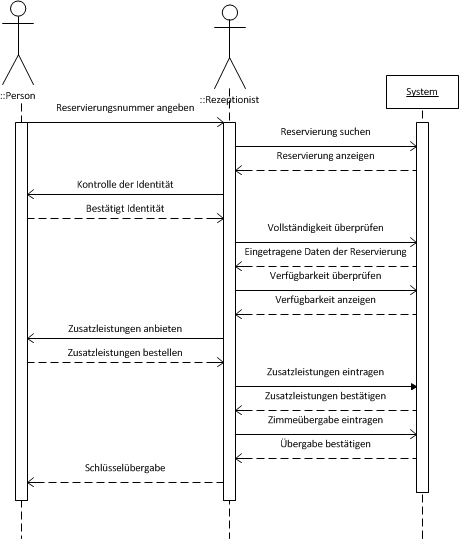
\includegraphics[width=\linewidth]{Images/SSD_Checkin_Reservierung.png}
	\caption{Checkin Reservierung - Sequenzdiagramm}
\end{figure}

\paragraph{Besondere Anforderungen}
\begin{itemize}
	\item keine
\end{itemize}

\paragraph{Benutzerfrequenz}
mehrmals täglich (sehr hoch)

\paragraph{Offene Punkte}
\begin{itemize}
	\item Umgang mit Überbuchungen
	\item Umgang mit ungereinigten Zimmer
\end{itemize}

\newpage

